\documentclass[12pt,letterpaper]{article}
\usepackage{fullpage}
\usepackage[top=2cm, bottom=4.5cm, left=2.5cm, right=2.5cm]{geometry}
\usepackage{amsmath,amsthm,amsfonts,amssymb,amscd}
\usepackage{lastpage}
\usepackage{enumerate}
\usepackage{fancyhdr}
\usepackage{mathrsfs}
\usepackage{xcolor}
\usepackage{fancyvrb}
\usepackage{graphicx}
\usepackage{listings}
\usepackage{float}
\usepackage{hyperref}
\usepackage{tikz}
\usepackage{relsize}
\usepackage{fancyvrb}
\usepackage{multirow}
\usepackage{booktabs}
\usepackage{import}
\usetikzlibrary{shapes.geometric,fit}

\hypersetup{%
  colorlinks=true,
  linkcolor=blue,
  linkbordercolor={0 0 1}
}

\setlength{\parindent}{0.0in}
\setlength{\parskip}{0.05in}

\theoremstyle{definition}
\newtheorem*{statement}{Statement}
\newtheorem*{claim}{Claim}
\newtheorem*{theorem}{Theorem}
\newtheorem*{lemma}{Lemma}

\newcommand{\contra}{\Rightarrow\!\Leftarrow}
\newcommand{\R}{\mathbb{R}}
\newcommand{\F}{\mathbb{F}}
\newcommand{\Z}{\mathbb{Z}}
\newcommand{\Zeq}{\mathbb{Z}_{\geq 0}}
\newcommand{\Zg}{\mathbb{Z}_{>0}}
\newcommand{\Req}{\mathbb{R}_{\geq 0}}
\newcommand{\Rg}{\mathbb{R}_{>0}}
\newcommand{\N}{\mathbb{N}}
\newcommand{\Q}{\mathbb{Q}}
\newcommand{\C}{\mathbb{C}}
\DeclareMathOperator{\Cov}{Cov}
\DeclareMathOperator{\Var}{Var}

\newcommand{\incfig}[1] {%
    \import{./figures/}{#1.pdf_tex}
}

\graphicspath{ {./figures/} }

\title{ECON 3412 HW 4}
\author{David Chen, dc3451}

\begin{document}

\maketitle

\section*{Problem 1}

The problem set uses the following function definition
\begin{Verbatim}[fontsize=\small]
robust_lm <- function(formula, data, conditions) {
  regression <- lm(formula, data = data)
  robust_coef <- coeftest(regression, vcov = vcovHC(regression, "HC1"))

  if (missing(conditions)) {
    return (list(regression, robust_coef))
  }

  f_test = linearHypothesis(regression, conditions, vcov = vcovHC(regression, "HC1"))

  return (list(regression, robust_coef, f_test))
}
\end{Verbatim}
which returns OLS regression, heteroskedacity robust standard errors, and a corresponding $F-$test on the hypotheses passed in \verb|conditions|.

\subsection*{a}

\begin{Verbatim}[fontsize=\small]
> summary(lm(formula = nettfa ~ p401k, data = read_dta("./401ksubs.dta")))

Call:
lm(formula = nettfa ~ p401k, data = read_dta("./401ksubs.dta"))

Residuals:
    Min      1Q  Median      3Q     Max
-513.97  -16.17  -11.57   -1.07 1498.33

Coefficients:
            Estimate Std. Error t value Pr(>|t|)
(Intercept)  11.6672     0.7669   15.21   <2e-16 ***
p401k        26.8057     1.4592   18.37   <2e-16 ***
---
Signif. codes:  0 ‘***’ 0.001 ‘**’ 0.01 ‘*’ 0.05 ‘.’ 0.1 ‘ ’ 1

Residual standard error: 62.83 on 9273 degrees of freedom
Multiple R-squared:  0.03512,	Adjusted R-squared:  0.03501
F-statistic: 337.5 on 1 and 9273 DF,  p-value: < 2.2e-16
\end{Verbatim}

The sign is positive with $p < 2e-16$. In particular, this suggests that on average, net total financial assests are higher among people with 401k's, by about 26.8 thousand dollars. This is not causal, as we did not impose any treatment or try to control for possible omitted variables.

\subsection*{b}

\begin{Verbatim}[fontsize=\small]
> summary(lm(formula = nettfa ~ p401k + e401k, data = read_dta("./401ksubs.dta")))

Call:
lm(formula = nettfa ~ p401k + e401k, data = read_dta("./401ksubs.dta"))

Residuals:
    Min      1Q  Median      3Q     Max
-513.92  -16.18  -11.58   -1.07 1498.33

Coefficients:
            Estimate Std. Error t value Pr(>|t|)
(Intercept) 11.67677    0.83687  13.953   <2e-16 ***
p401k       26.85585    2.28348  11.761   <2e-16 ***
e401k       -0.05965    2.09127  -0.029    0.977
---
Signif. codes:  0 ‘***’ 0.001 ‘**’ 0.01 ‘*’ 0.05 ‘.’ 0.1 ‘ ’ 1

Residual standard error: 62.84 on 9272 degrees of freedom
Multiple R-squared:  0.03512,	Adjusted R-squared:  0.03491
F-statistic: 168.7 on 2 and 9272 DF,  p-value: < 2.2e-16
\end{Verbatim}

We have a few cases:
\begin{enumerate}
  \item $p401k = 0, e401k = 1$. In this case, this is the set of people eligible but do not have a 401k.
  \item $p401k = 0, e401k = 0$. In this case, this is the set of people not eligible for a 401k (and thus do not have one).
  \item $p401k = 1, e401k = 1$. In this case, this is the set of people eligible and containing a 401k.
  \item $p401k = 1, e401k = 0$. This makes no interpretive sense, as noone who has a 401k is ineligible for one.
\end{enumerate}

In particular, $e401k$ is not significantly different from 0, so we can't reject the null that it has no effect on net financial assets. Even if it were significantly negative, the fourth category makes interpretation hard, with a negative coefficient not necessarily implying that eligibility lowers assets, since it is not meaningful to hold $p401k = 1$ constant and change $e401k$ between $0$ and $1$.

\subsection*{c}

\begin{Verbatim}[fontsize=\small]
> summary(lm(formula = nettfa ~ p401k + age + agesq + fsize + inc + incsq +
             male + marr, data = read_dta("./401ksubs.dta")))

Call:
lm(formula = nettfa ~ p401k + age + agesq + fsize + inc + incsq +
    male + marr, data = read_dta("./401ksubs.dta"))

Residuals:
    Min      1Q  Median      3Q     Max
-512.80  -16.03   -2.85    6.55 1459.05

Coefficients:
              Estimate Std. Error t value Pr(>|t|)
(Intercept) 20.6413058 10.0331658   2.057 0.039685 *
p401k       15.8385887  1.3806608  11.472  < 2e-16 ***
age         -1.6592052  0.4958743  -3.346 0.000823 ***
agesq        0.0311596  0.0057074   5.460  4.9e-08 ***
fsize       -1.2747034  0.4961944  -2.569 0.010216 *
inc         -0.2402240  0.0778799  -3.085 0.002045 **
incsq        0.0099437  0.0005939  16.742  < 2e-16 ***
male         0.6864445  1.6056200   0.428 0.669006
marr        -2.8620618  1.6912574  -1.692 0.090628 .
---
Signif. codes:  0 ‘***’ 0.001 ‘**’ 0.01 ‘*’ 0.05 ‘.’ 0.1 ‘ ’ 1

Residual standard error: 56.86 on 9266 degrees of freedom
Multiple R-squared:  0.2105,	Adjusted R-squared:  0.2098
F-statistic: 308.8 on 8 and 9266 DF,  p-value: < 2.2e-16
\end{Verbatim}

\begin{enumerate}
  \item Holding 401k participation, age, income, gender, and marriage status constant, a unit increase in family size is associated with a significant decrease in net assets of about 1.27 thousand dollars.
  \item Holding 401k participation, age, family size, income, and marriage status constant, men on average have higher net assests by about 686 dollars (though not statistically significant).
  \item Holding 401k participation, age, family size, income, and gender constant, married people usually have lower net financial assets by about 2.86 thousand dollars (though not statistically significant).
  \item Holding age, family size, income, gender, and marriage status constant, 401k participation is associated with an increase in net assests of 15.8k thousand dollars.
  \item Holding 401k participation, family size, income, gender, and marriage status constant, the coefficient of the square of age being significantly positive gives that net assests is convex w.r.t age, meaning that it troughs at some age before recovering.
\end{enumerate}

The coefficient on p401k is still positive and significant, but has decreased significantly. We still cannot treat p401k as causal without further analysis, since there are still potential omitted variables such as something like education which is likely correlated positively with net assets and 401k participation and may be incompletely controlled for by the controls like income. However, we are at the very least probably much closer to the true effect of p401k participation on net assets.

\subsection*{d}

\begin{Verbatim}[fontsize=\small]
> robust_lm(nettfa ~ p401k + age + agesq + fsize + inc +
              incsq + male + marr + I(age * male) + I(agesq * male) +
              I(fsize * male) + I(inc * male) + I(incsq * male) + I(marr * male),
            read_dta("./401ksubs.dta"),
            c("I(age * male) = 0", "I(agesq * male) = 0", "I(fsize * male) = 0",
                  "I(inc * male) = 0", "I(incsq * male) = 0", "I(marr * male) = 0"))

t test of coefficients:

                   Estimate  Std. Error t value  Pr(>|t|)
(Intercept)      22.9791554  12.7679611  1.7998 0.0719324 .
p401k            15.6001277   1.5691764  9.9416 < 2.2e-16 ***
age              -1.6243755   0.5542565 -2.9307 0.0033899 **
agesq             0.0302862   0.0068401  4.4278 9.631e-06 ***
fsize            -1.5843633   0.4273087 -3.7078 0.0002103 ***
inc              -0.3979227   0.3381638 -1.1767 0.2393391
incsq             0.0115973   0.0033362  3.4762 0.0005108 ***
male            -11.0138861  35.3309684 -0.3117 0.7552492
marr             -0.7138830   1.8277232 -0.3906 0.6961123
I(age * male)    -0.4394884   1.9142040 -0.2296 0.8184129
I(agesq * male)   0.0076310   0.0249049  0.3064 0.7593016
I(fsize * male)   2.2555591   1.2949886  1.7418 0.0815837 .
I(inc * male)     0.9637646   0.4075266  2.3649 0.0180548 *
I(incsq * male)  -0.0106100   0.0039353 -2.6961 0.0070274 **
I(marr * male)  -10.0546811   4.8362413 -2.0790 0.0376422 *
---
Signif. codes:  0 ‘***’ 0.001 ‘**’ 0.01 ‘*’ 0.05 ‘.’ 0.1 ‘ ’ 1

Linear hypothesis test

Hypothesis:
I(age * male) = 0
I(agesq * male) = 0
I(fsize * male) = 0
I(inc * male) = 0
I(incsq * male) = 0
I(marr * male) = 0

Model 1: restricted model
Model 2: nettfa ~ p401k + age + agesq + fsize + inc + incsq + male + marr +
    I(age * male) + I(agesq * male) + I(fsize * male) + I(inc *
    male) + I(incsq * male) + I(marr * male)

Note: Coefficient covariance matrix supplied.

  Res.Df Df      F   Pr(>F)
1   9266
2   9260  6 3.0597 0.005427 **
---
Signif. codes:  0 ‘***’ 0.001 ‘**’ 0.01 ‘*’ 0.05 ‘.’ 0.1 ‘ ’ 1
\end{Verbatim}

\begin{enumerate}
  \item The coefficient on $p401k$ still is interpreted to be that holding all the other controls, we expect that someone with a 401k is on average 15.6 thousand dollars wealthier in terms of net total financial assets.
  \item The coefficient of $fsize * male$ can be interpreted as holding all else constant, the difference of the effect a unit change in the family size will affect net fin assets between men and women, i.e. men expect to see 2.25 thousand more per family member than women.
  \item The coefficient of $marr * male$ can be interpreted as holding all else constant, the difference of the difference average unmarried and married man and average unmarried and married woman, i.e. we expect that the gap between married and unmarried men is 10 thousand smaller than the gap between married and unmarried women.
\end{enumerate}

We have that the joint null hypothesis that all of the interactions are zero is rejected at the 1\% level with $p = 0.005$.

This means that the control variables do interact differently for men than for women, particularly income (which matches with the wage gap that we would expect to see). We still can't tell if the coefficient is causal for the same reason as before, as we still cannot be certain that there are no omitted factors (though, as before, we could make a judgment call). In fact, we are probably even more convinced that it is not causal, as we have that we cannot predict nettfa accurately without knowing gender.

\subsection*{e}

\begin{Verbatim}[fontsize=\small]
> robust_lm(nettfa ~ p401k + age + agesq + fsize + inc +
              incsq + male + marr + I(p401k * male) + I(age * male) + I(agesq * male) +
              I(fsize * male) + I(inc * male) + I(incsq * male) + I(marr * male),
            read_dta("./401ksubs.dta"))

t test of coefficients:

                   Estimate  Std. Error t value  Pr(>|t|)
(Intercept)      22.7546594  12.7474554  1.7850 0.0742883 .
p401k            14.9264851   1.7292610  8.6317 < 2.2e-16 ***
age              -1.6129615   0.5535375 -2.9139 0.0035778 **
agesq             0.0301541   0.0068326  4.4133  1.03e-05 ***
fsize            -1.5887474   0.4270936 -3.7199 0.0002005 ***
inc              -0.3912893   0.3376781 -1.1588 0.2465822
incsq             0.0115706   0.0033337  3.4708 0.0005212 ***
male            -10.2901958  34.9897490 -0.2941 0.7686944
marr             -0.7296842   1.8270755 -0.3994 0.6896278
I(p401k * male)   3.4481089   4.0975782  0.8415 0.4000901
I(age * male)    -0.4723996   1.9009430 -0.2485 0.8037469
I(agesq * male)   0.0080428   0.0247445  0.3250 0.7451623
I(fsize * male)   2.2848430   1.3006458  1.7567 0.0790022 .
I(inc * male)     0.9237757   0.3995816  2.3119 0.0208074 *
I(incsq * male)  -0.0104071   0.0039055 -2.6647 0.0077190 **
I(marr * male)   -9.9864083   4.8010676 -2.0800 0.0375494 *
---
Signif. codes:  0 ‘***’ 0.001 ‘**’ 0.01 ‘*’ 0.05 ‘.’ 0.1 ‘ ’ 1
\end{Verbatim}

The regression implies that holding the other controls constant, we expect to see that on average, women with a 401k have higher net assets by 14.9k than other women, whereas men with a 401k have higher assets of $14.9 + 3.45 = 18.35$ thousand than other men.

\verb|xs[[1]]| is the above regression in the following lines.

Testing whether the effect for men is $0$, we get
\begin{Verbatim}[fontsize=\small]
> linearHypothesis(xs[[1]], c("p401k = -I(p401k * male)"), vcov = vcovHC(xs[[1]], type = "HC1"))
Linear hypothesis test

Hypothesis:
p401k  + I(p401k * male) = 0

Model 1: restricted model
Model 2: nettfa ~ p401k + age + agesq + fsize + inc + incsq + male + marr +
    I(p401k * male) + I(age * male) + I(agesq * male) + I(fsize *
    male) + I(inc * male) + I(incsq * male) + I(marr * male)

Note: Coefficient covariance matrix supplied.

  Res.Df Df      F    Pr(>F)
1   9260
2   9259  1 24.466 7.696e-07 ***
---
Signif. codes:  0 ‘***’ 0.001 ‘**’ 0.01 ‘*’ 0.05 ‘.’ 0.1 ‘ ’ 1
\end{Verbatim}
Thus, we reject that the effect for men is 0.

Testing whether the effect for women is $0$, we get
\begin{Verbatim}[fontsize=\small]
> linearHypothesis(xs[[1]], c("p401k = 0"), vcov = vcovHC(xs[[1]], type = "HC1"))
Linear hypothesis test

Hypothesis:
p401k = 0

Model 1: restricted model
Model 2: nettfa ~ p401k + age + agesq + fsize + inc + incsq + male + marr +
    I(p401k * male) + I(age * male) + I(agesq * male) + I(fsize *
    male) + I(inc * male) + I(incsq * male) + I(marr * male)

Note: Coefficient covariance matrix supplied.

  Res.Df Df      F    Pr(>F)
1   9260
2   9259  1 74.507 < 2.2e-16 ***
---
Signif. codes:  0 ‘***’ 0.001 ‘**’ 0.01 ‘*’ 0.05 ‘.’ 0.1 ‘ ’ 1
\end{Verbatim}
Thus, we reject that the effect for women is 0.

Testing whether they are the same,
\begin{Verbatim}[fontsize=\small]
> linearHypothesis(xs[[1]], c("I(p401k * male) = 0"), vcov = vcovHC(xs[[1]], type = "HC1"))
Linear hypothesis test

Hypothesis:
I(p401k * male) = 0

Model 1: restricted model
Model 2: nettfa ~ p401k + age + agesq + fsize + inc + incsq + male + marr +
    I(p401k * male) + I(age * male) + I(agesq * male) + I(fsize *
    male) + I(inc * male) + I(incsq * male) + I(marr * male)

Note: Coefficient covariance matrix supplied.

  Res.Df Df      F Pr(>F)
1   9260
2   9259  1 0.7081 0.4001
\end{Verbatim}
so we cannopt reject that the effects are the same.

\section*{Problem 2}

\subsection*{a}

\verb|> ggplot(terror_dta, aes(x=gdppc, y=ftmpop)) + geom_point() + ylim(0,5)|
\begin{center}
  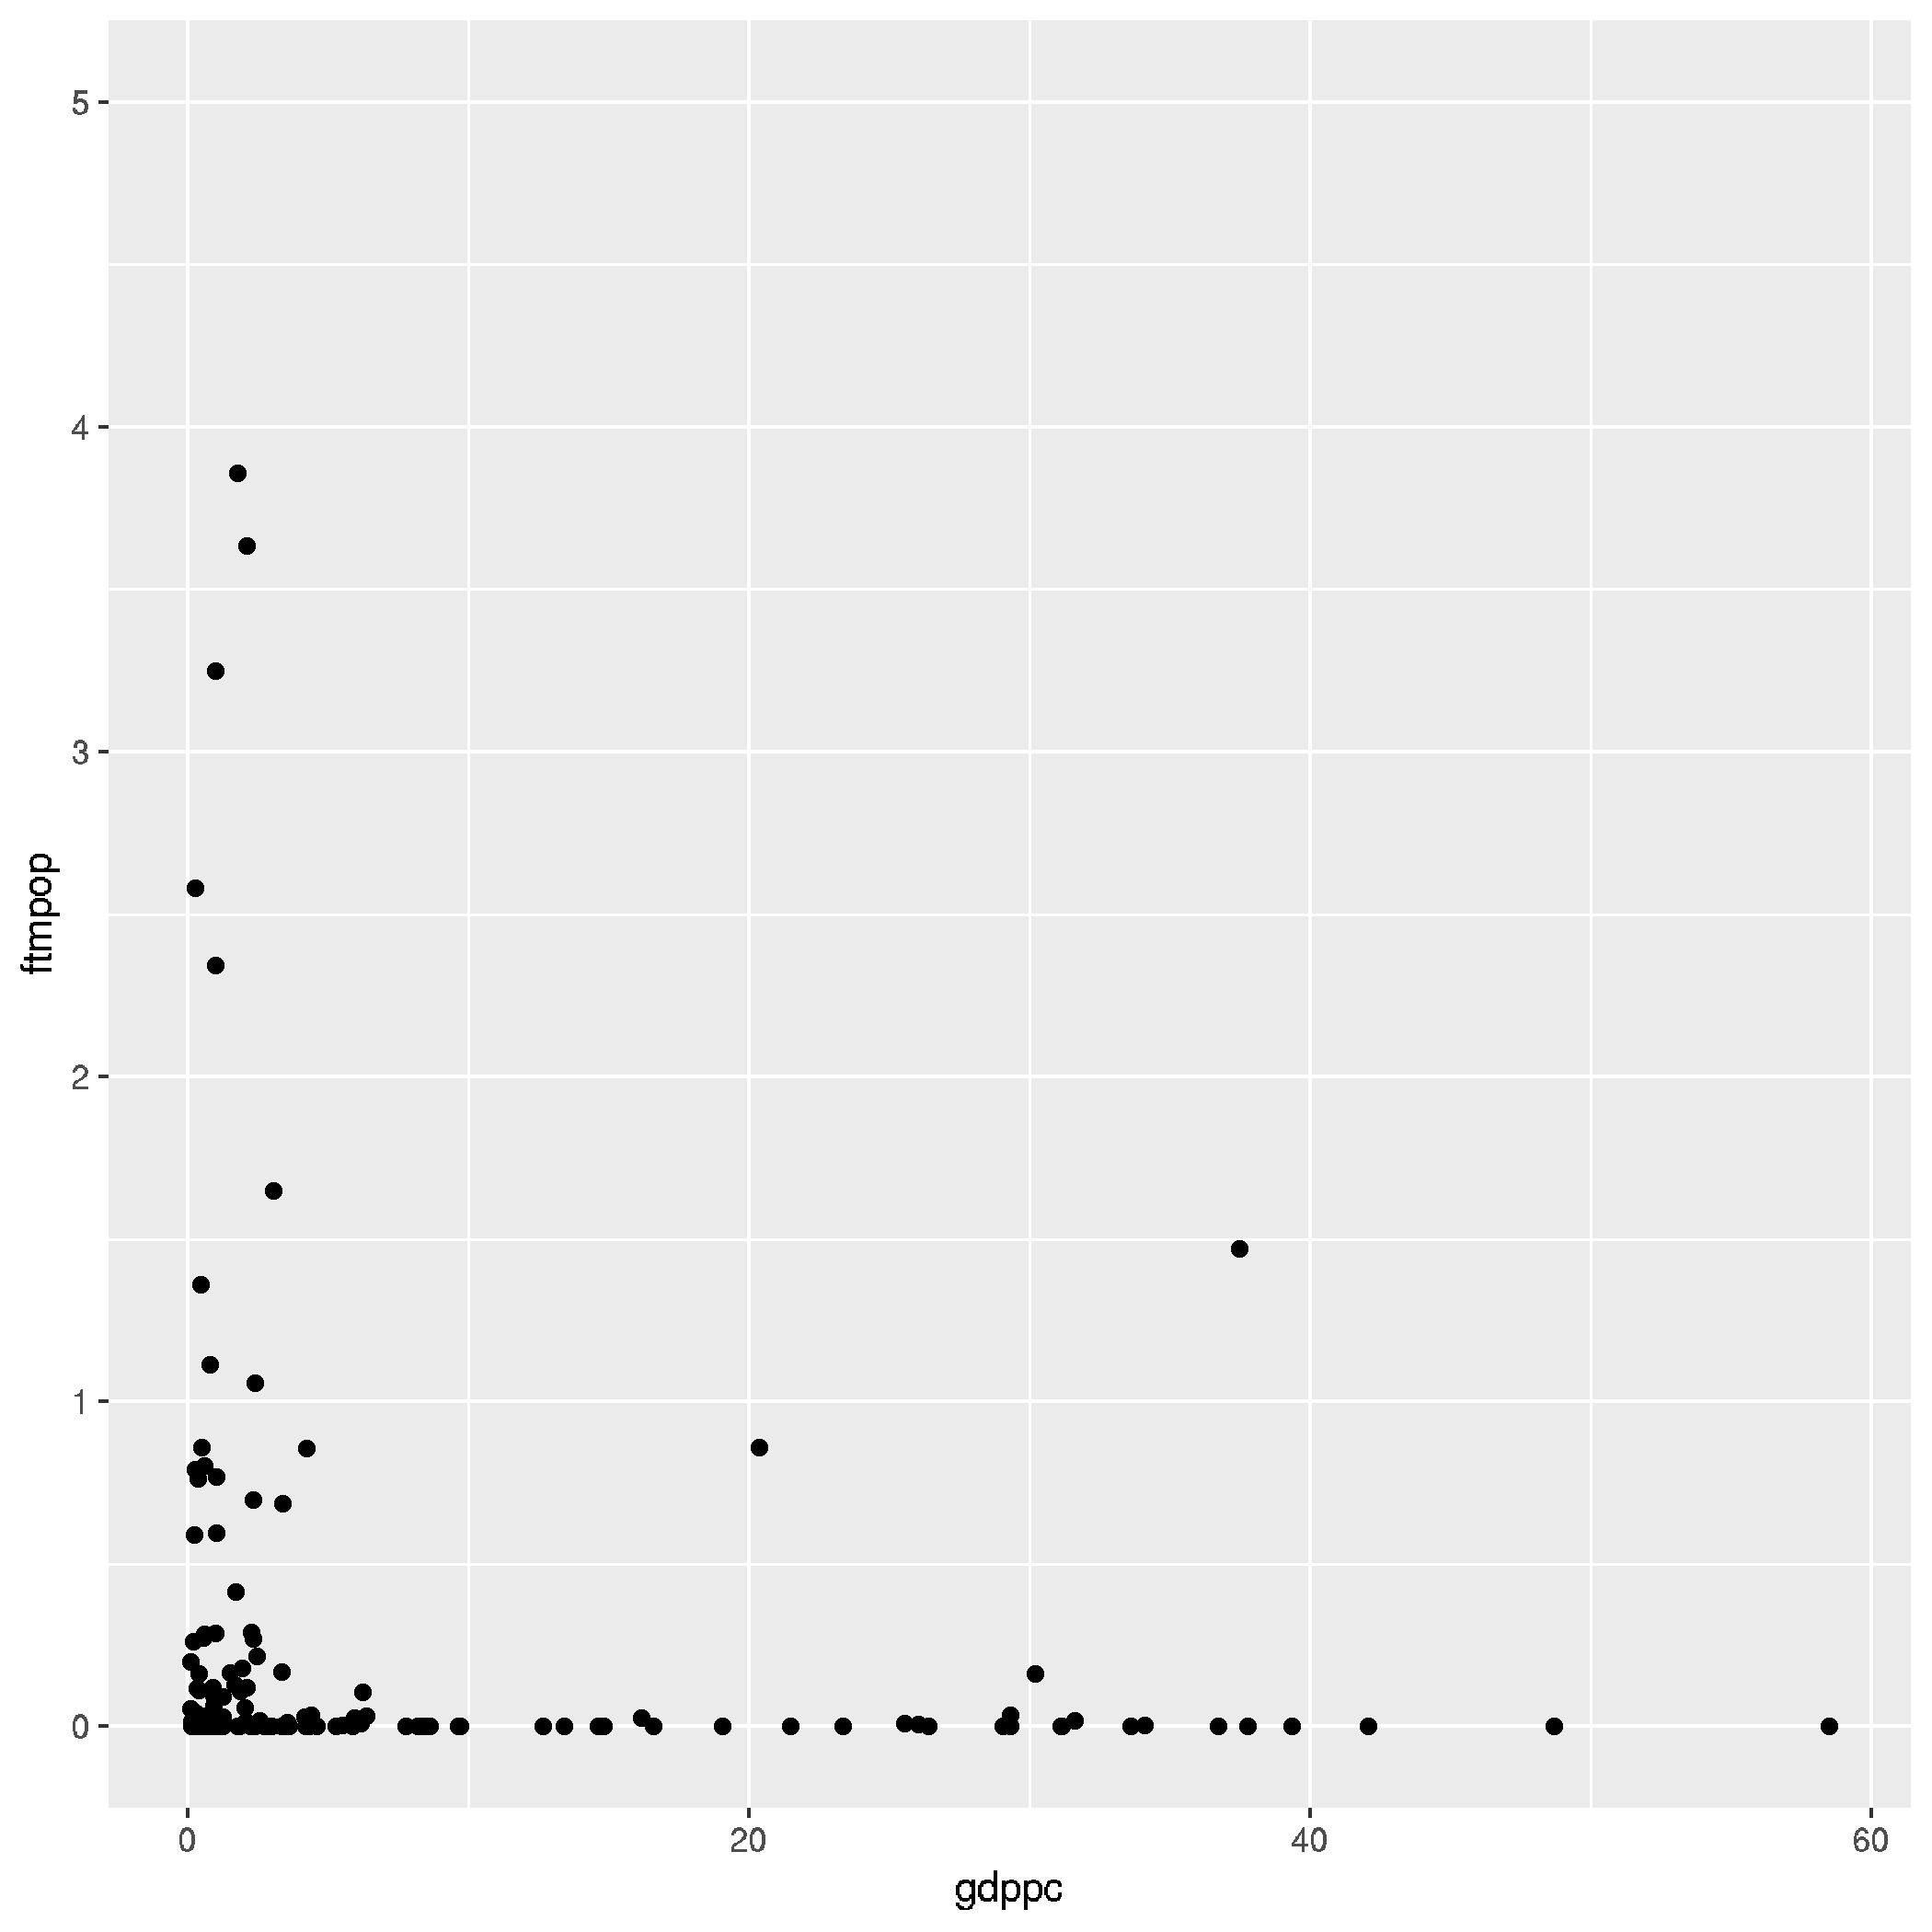
\includegraphics[width=0.6\textwidth]{figures/2a.png}
\end{center}

\subsection*{b}
\verb|> ggplot(terror_dta, aes(x=log(gdppc), y=log(ftmpop))) + geom_point()|
\begin{center}
  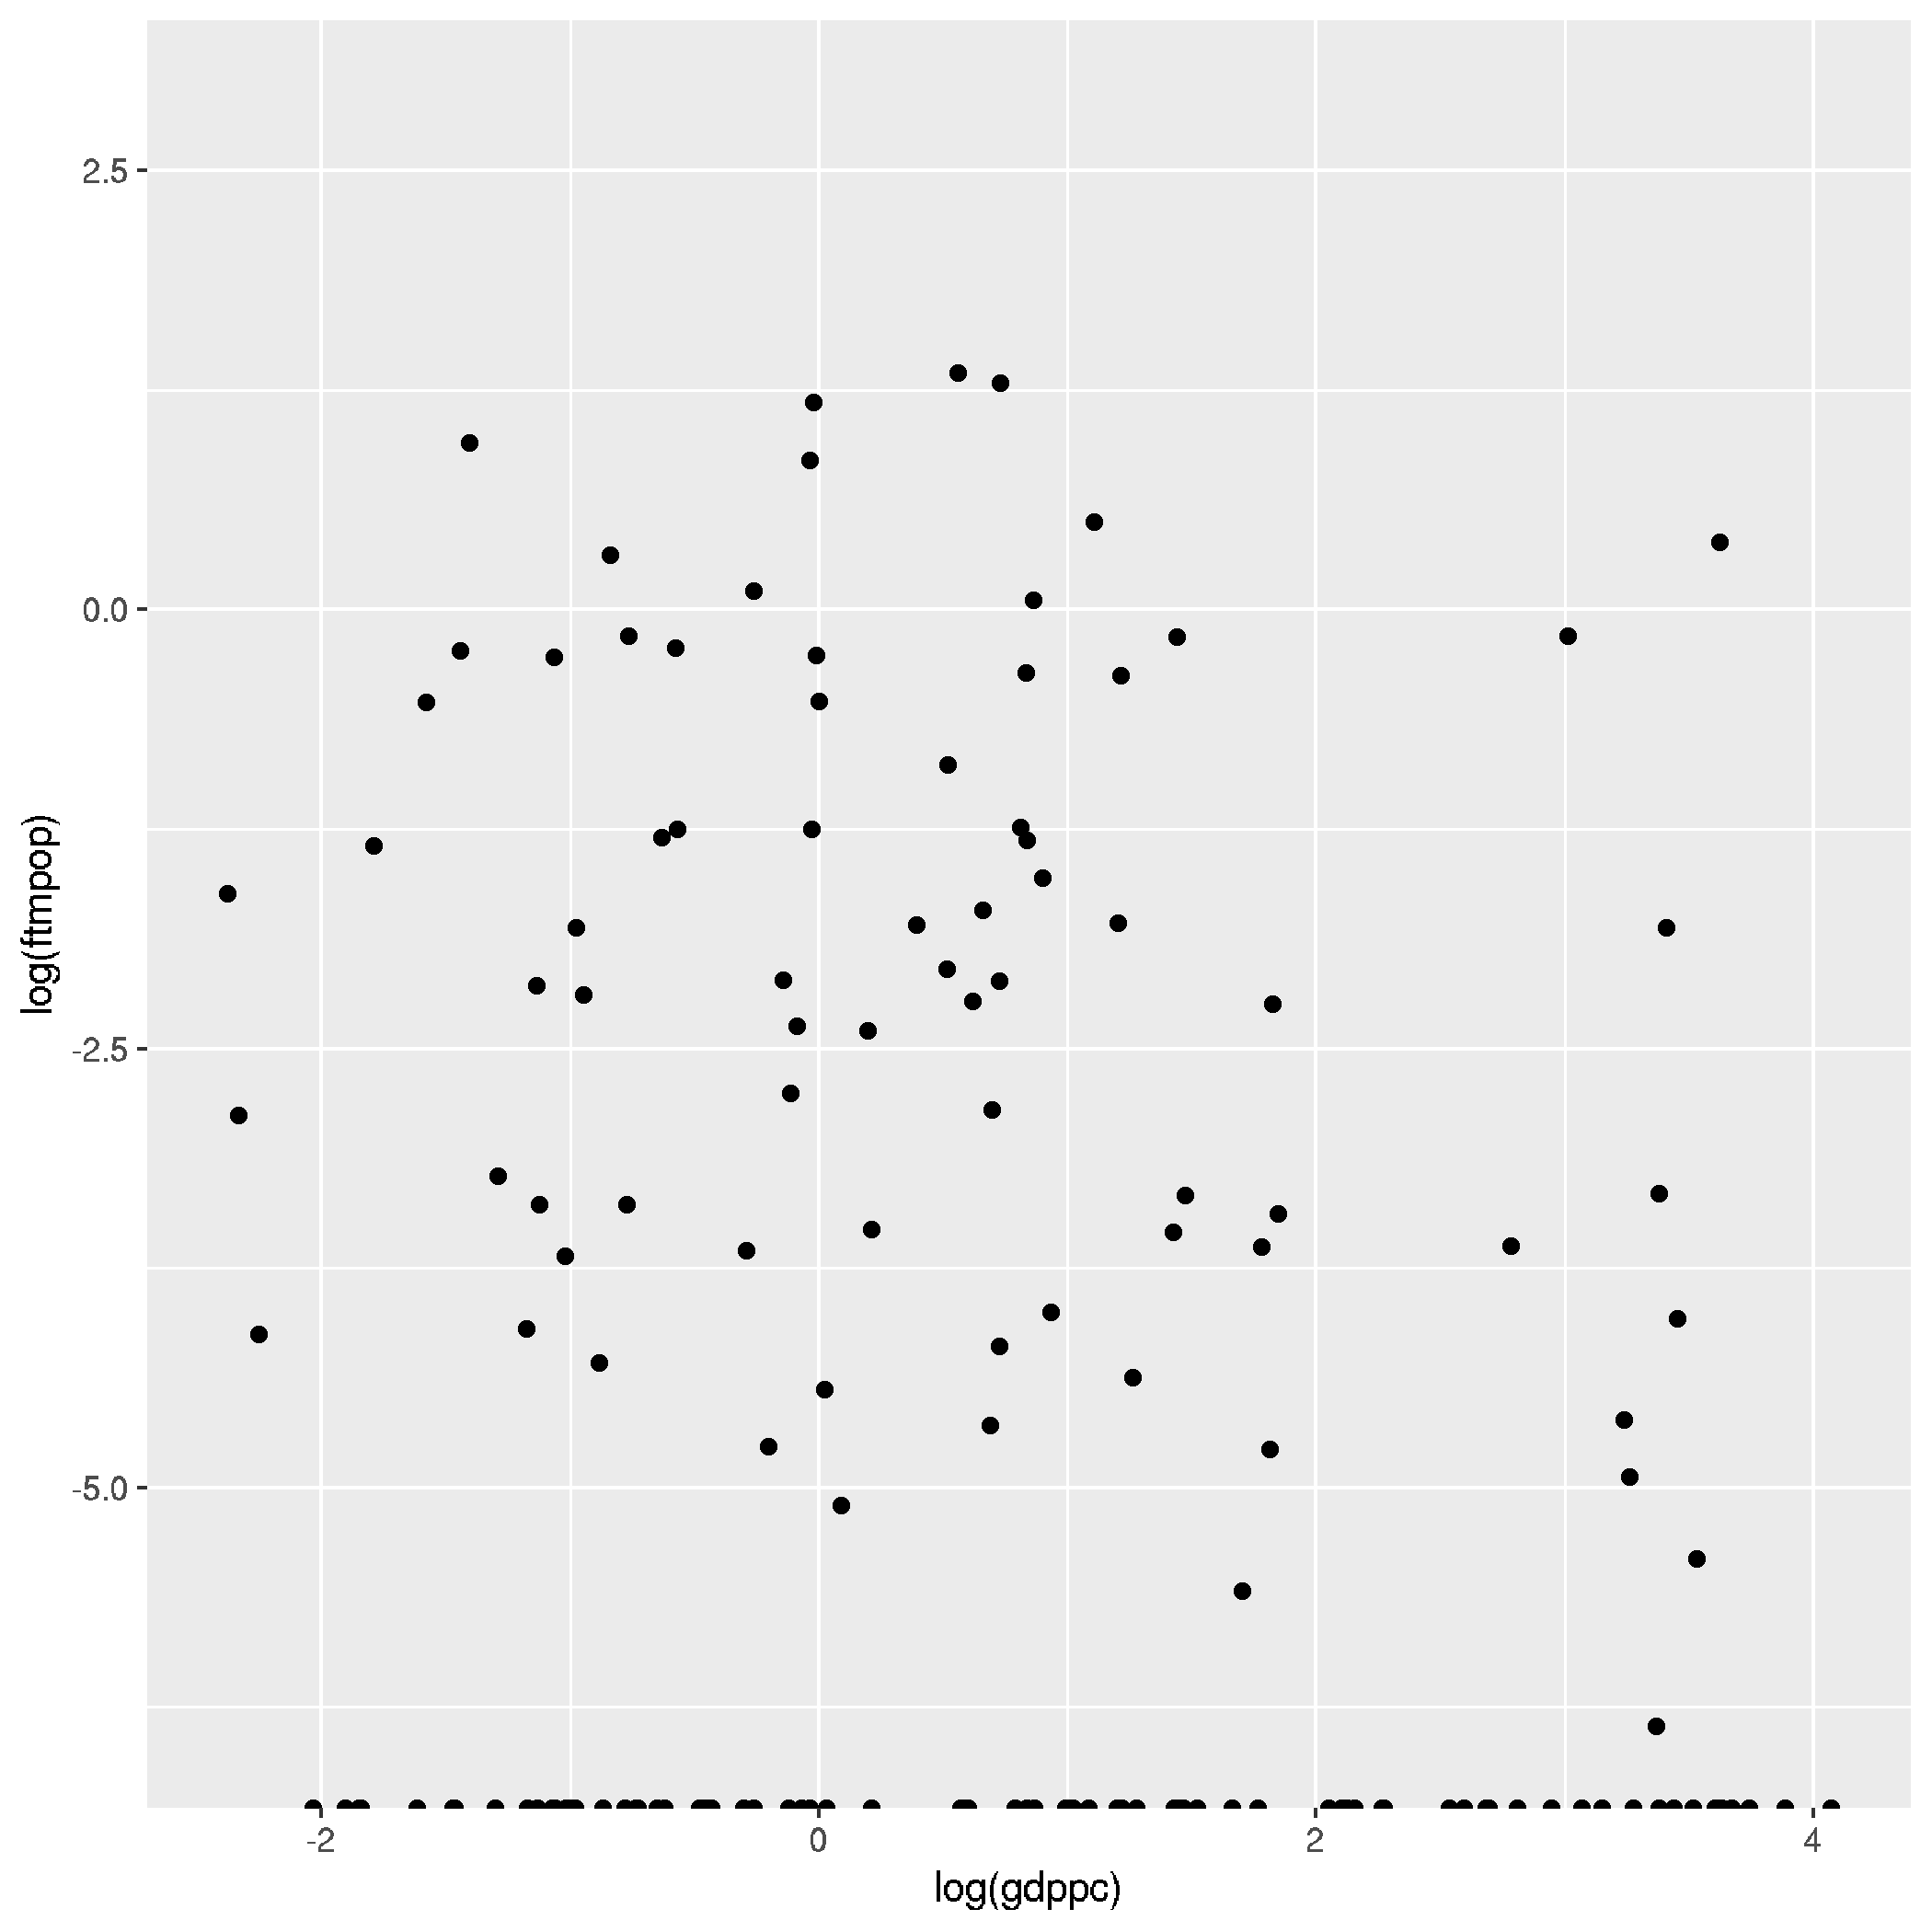
\includegraphics[width=0.6\textwidth]{figures/2b.png}
\end{center}
\subsection*{c}
\verb|> ggplot(terror_dta, aes(x=lackpf, y=log(ftmpop))) + geom_point()|
\begin{center}
  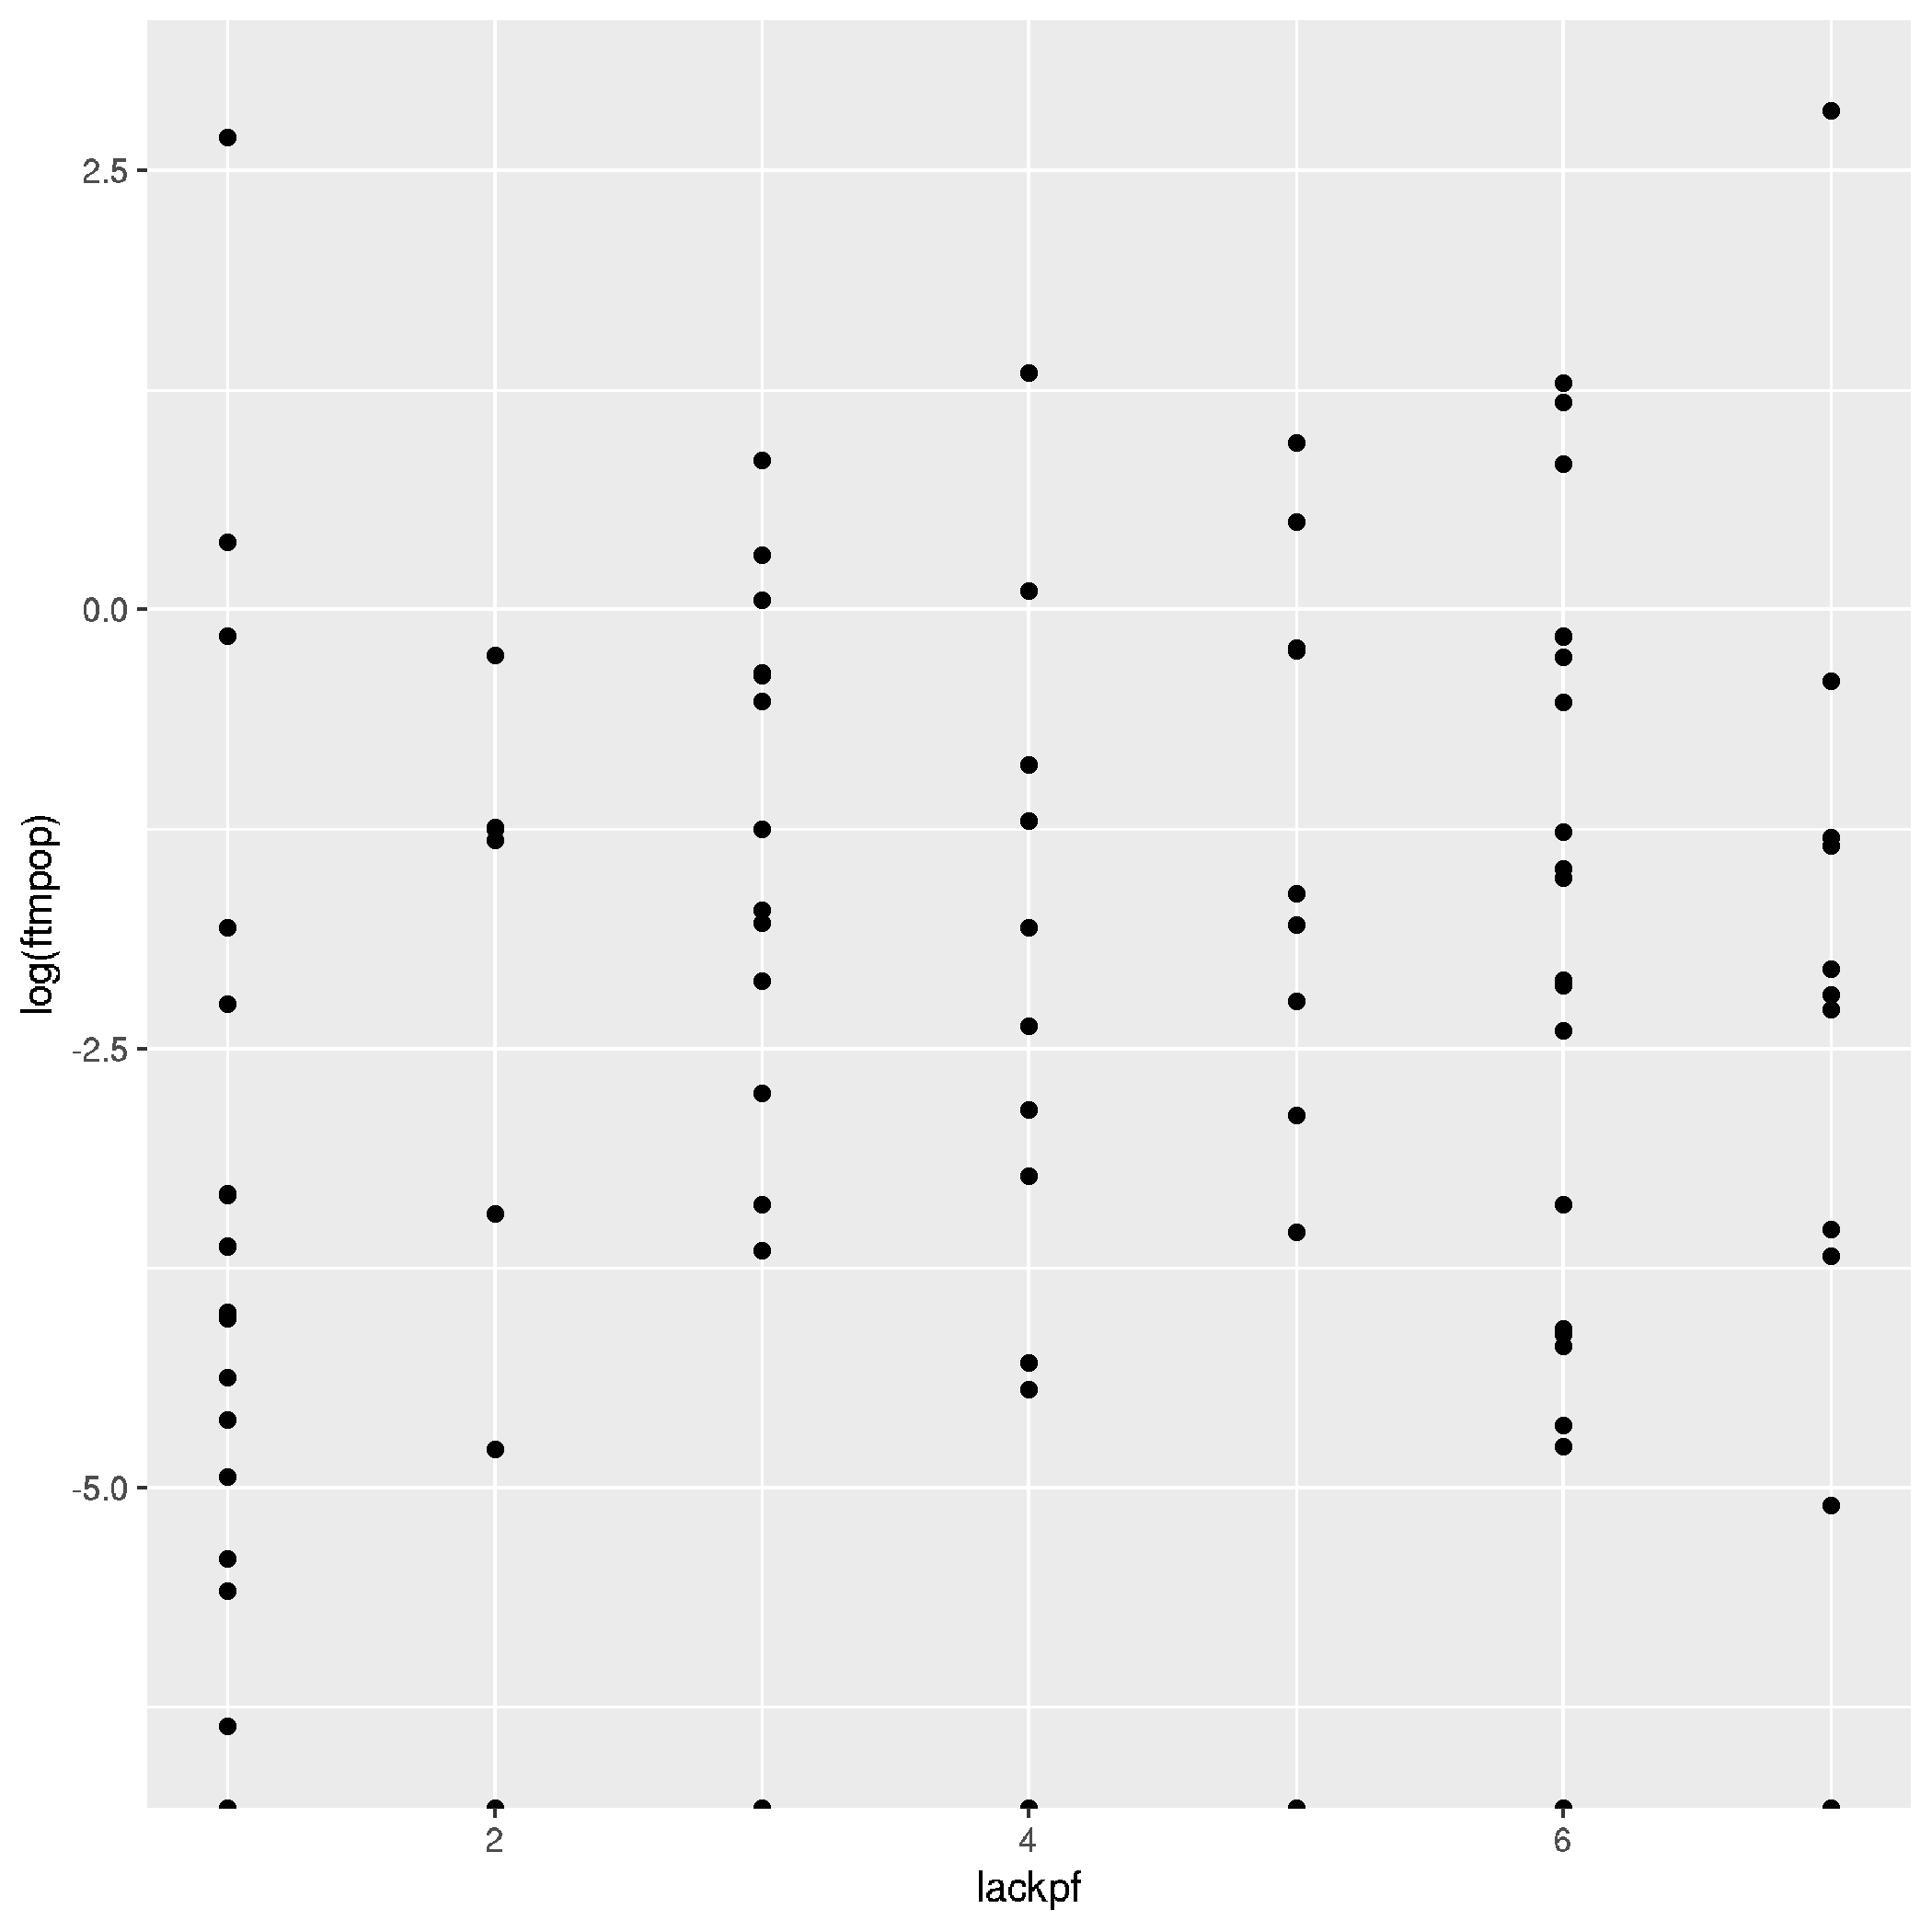
\includegraphics[width=0.6\textwidth]{figures/2c.png}
\end{center}
\subsection*{d}

The scatter plot from a looks heavily nonlinear, with data clustered on the axes. The second one, once countries with $ftmpop = 0$ are cleaned, looks much better to regress on, so we prefer $lnftmpop$ v $lngpdpc$.

\subsection*{e}

The scatterplot is a little too disparate to tell. It could be linear with a decent amount of heteroskedacity, and it is too unclear to say much more, though it does curve up in the middle, suggesting something like a quadratic fit.

\section*{Problem 3}

We first remove the countries with 0 $ftmppop$ by

\verb|> terror_dta <- read_dta("./terrorism.dta")|

\verb|> terror_dta <- terror_dta[terror_dta$ftmpop != 0,]|

We then have the following:

\begin{center}
  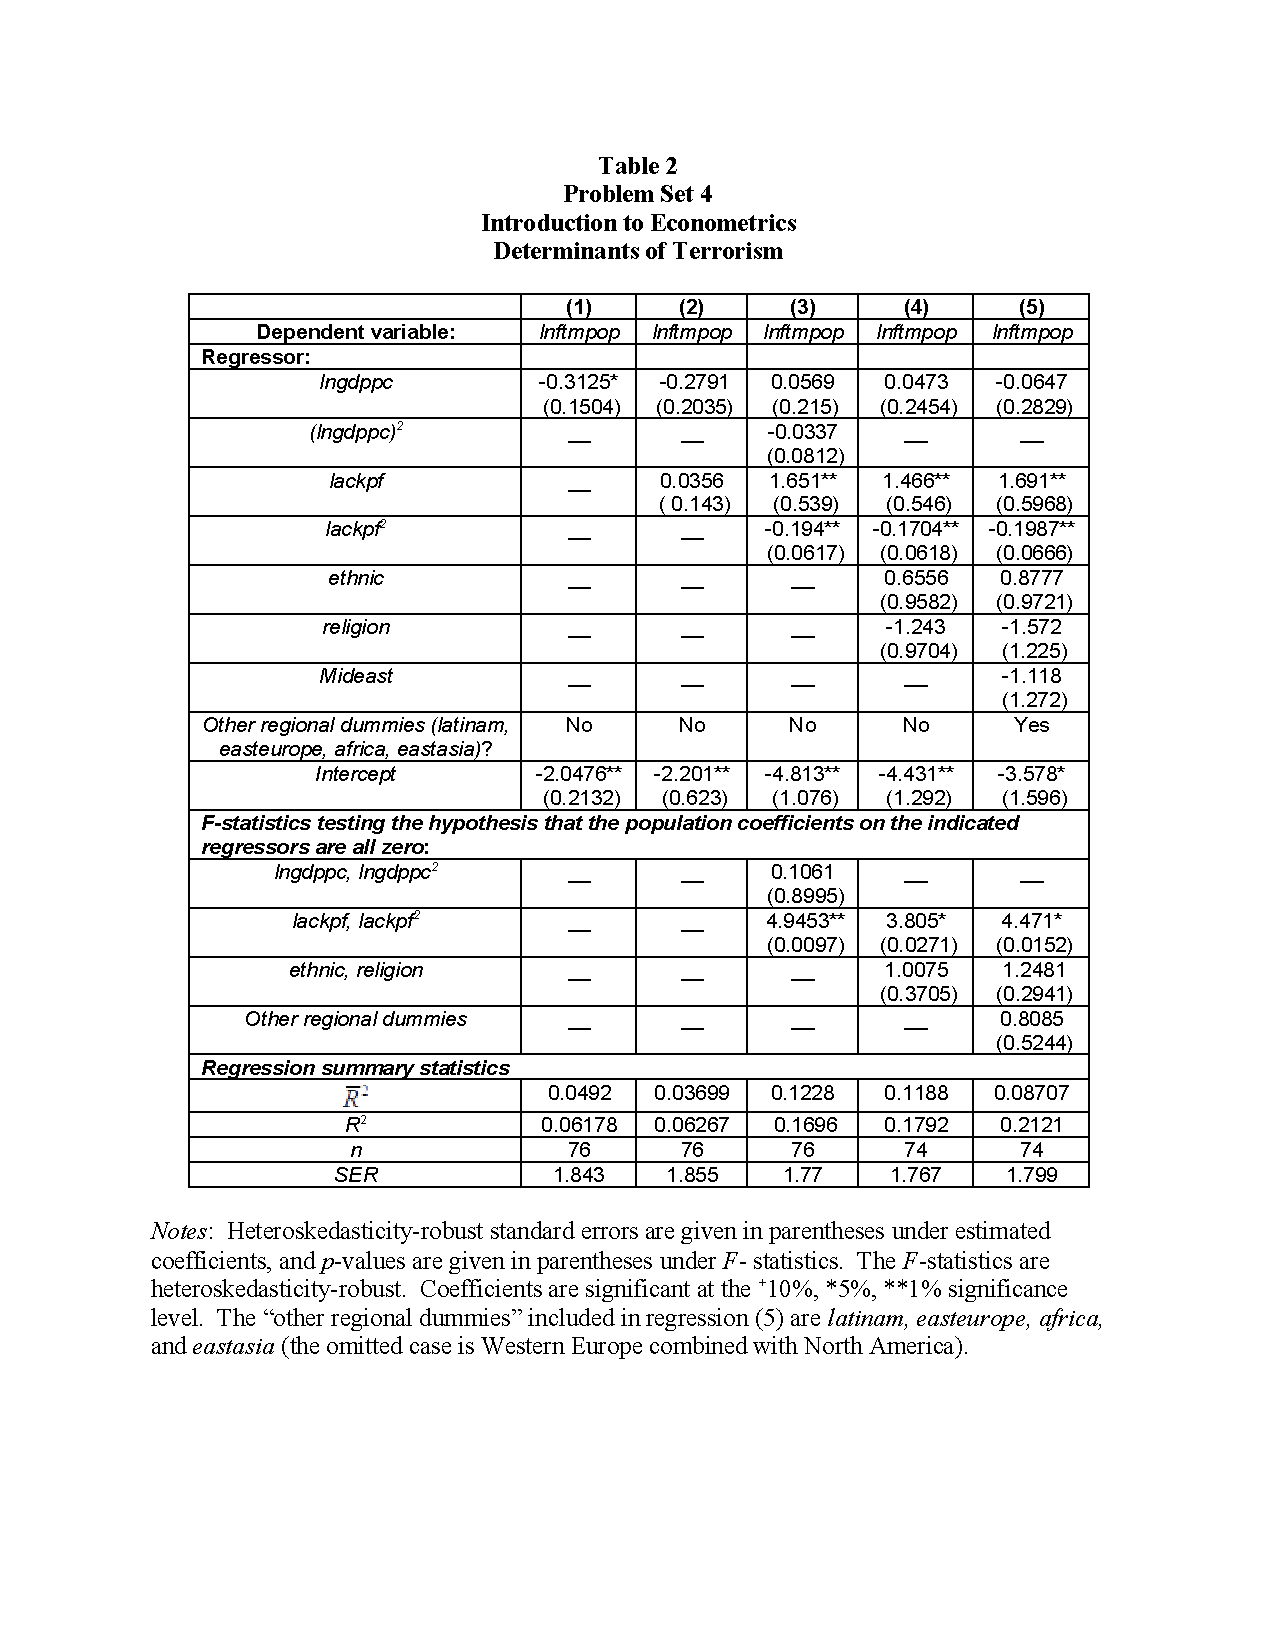
\includegraphics[width=\textwidth]{./figures/table2.pdf}
\end{center}
which is given by the following \verb|R|
\begin{Verbatim}[fontsize=\small]
terror_dta <- read_dta("./terrorism.dta")
terror_dta <- terror_dta[terror_dta$ftmpop != 0,]
terror_dta$lnftmpop <- log(terror_dta$ftmpop)
terror_dta$lngdppc <- log(terror_dta$gdppc)

t2_reg = list()
t2_reg[[1]] <- robust_lm(lnftmpop ~ lngdppc, terror_dta)
t2_reg[[2]] <- robust_lm(lnftmpop ~ lngdppc + lackpf, terror_dta)
t2_reg[[3]] <- robust_lm(lnftmpop ~ lngdppc + I(lngdppc ^ 2) +
                           lackpf + I(lackpf ^ 2), terror_dta)
t2_reg[[4]] <- robust_lm(lnftmpop ~ lngdppc + lackpf +
                           I(lackpf ^ 2) + ethnic + religion, terror_dta)
t2_reg[[5]] <- robust_lm(lnftmpop ~ lngdppc + lackpf +
                           I(lackpf ^ 2) + ethnic + religion +
                           mideast + latinam + easteurope + africa + eastasia,
                         terror_dta)

linearHypothesis(t2_reg[[3]][[1]],
                 c("lngdppc = 0", "I(lngdppc^2) = 0"),
                 vcov = vcovHC(t2_reg[[3]][[1]], "HC1"))
linearHypothesis(t2_reg[[3]][[1]],
                 c("lackpf = 0", "I(lackpf^2) = 0"),
                 vcov = vcovHC(t2_reg[[3]][[1]], "HC1"))
linearHypothesis(t2_reg[[4]][[1]],
                 c("lackpf = 0", "I(lackpf^2) = 0"),
                 vcov = vcovHC(t2_reg[[4]][[1]], "HC1"))
linearHypothesis(t2_reg[[4]][[1]],
                 c("ethnic = 0", "religion = 0"),
                 vcov = vcovHC(t2_reg[[4]][[1]], "HC1"))
linearHypothesis(t2_reg[[5]][[1]],
                 c("lackpf = 0", "I(lackpf^2) = 0"),
                 vcov = vcovHC(t2_reg[[5]][[1]], "HC1"))
linearHypothesis(t2_reg[[5]][[1]],
                 c("ethnic = 0", "religion = 0"),
                 vcov = vcovHC(t2_reg[[5]][[1]], "HC1"))
linearHypothesis(t2_reg[[5]][[1]],
                 c("latinam = 0", "easteurope = 0", "africa = 0", "eastasia = 0"),
                 vcov = vcovHC(t2_reg[[5]][[1]], "HC1"))
\end{Verbatim}

\section*{Problem 4}

\subsection*{a}

This is significant at the $p = 0.05$ level. In fact, we can compute the t-statistic to be $-0.3125 / 0.1504 = -2.077$, so this is significant at $p = 2(1 - \Phi(2.077) = 0.377$.

This means that when all the other controls are help constant, a $1\%$ change in gdp/capita will be associated with a decrease in the fatalities from terrorism by $0.3125\%$.

\subsection*{b}

This is insignificant with $F-$statistic $0.1061$ and $p = 0.8995 > 0.05$, as seen in the table.

\subsection*{c}

Including $lackpf$ as a regressor also changes the calculated effect of $lngdppc$ as well, as they are likely correlated, with richer countries tending to be more free, and both determine terrorism, so $lngdppc$ and $lngdppc^{2}$ turn out to be a lot less well-estimated after accounting for religious freedom.

\subsection*{d}

No, the coefficient of $lngpdpc^{2}$ is not significantly different from 0, as seen in the table.

\subsection*{e}

Yes, the coefficient of $lackpf^{2}$ is significantly different from 0, as seen in the table, and is significant at the $1\%$ level, so there is evidence for nonlinearity.

\subsection*{f}

The $F-$test is carried out in the table, with $F = 0.8085$, $p = 0.5244$. We cannot reject the joint hypothesis all of the coefficients of the dummies vanish. The amount of restrictions is $q = 4$, and the critical value is then (where $qf$ is the quantile function of $F_{4,\infty}$) $qf(0.95) = 2.372$.

\subsection*{g}

The coefficient on $ethnic$ is not significantly different from 0 (see table), so we cannot reject the null that there is no effect of ethnic diversity on terrorist violence. The coefficient does suggest that we expect that increasing the ethnic fractionalization is associated with an increase in terrorist violence however. A more quantitaive description is too hard to give given the vague description of $ethnic$ in the homework.

\subsection*{h}

The coefficient on $religion$ is not significantly different from 0 (see table), so we cannot reject the null that there is no effect of religious diversity on terrorist violence. The coefficient does suggest that we expect that increasing the religious fractionalization is associated with a decrease in terrorist violence however. A more quantitaive description is too hard to give given the vague description of $religion$ in the homework.


\subsection*{i}

The $F-$test is conducted in the table, with $F=1.0075$, $p =0.3705$. We cannot reject the null that the coefficients on $ethnic$ and $religion$ are both $0$ (and thus that terrorism is unassociated with ethnic and religious diversity) at a standard $5\%$ level. Since we don't reject, we do not have statistically significant evidence that terrorism is associated with ethnic and religious diversity. In particular, we tested
\[
  H_{0}: \beta_{ethnic} = \beta_{religion} = 0, H_{1}: \text{ at least one of } \beta_{ethnic}, \beta_{religion} \neq 0
\]

\subsection*{j}

No. The homoskedasticity only $F-$test relies on the restricted model (here, regression 4) differing from the unrestricted model only by setting the coefficients as in the null; however, regression 3 also regresses on $lngdppc$ as well, so we cannot use these two to test the same joint hypothesis as i.

\subsection*{k}

The effect should be that $lnftmpop$ should change by $(1.691(7) - 0.1987(7)^{2}) - (1.691(5) - 0.1987(5)^{2}) = -1.3868$. Thus, $lnftmpop$ should actually increase by 1.3868 as a result from taking $lackpf$ from $7 \rightarrow 5$.

\subsection*{l}

This is approximately maximized when, taking the first derivative, $1.691 - 0.1987(2 * lackpf) = 0$, so $lackpf = 4.255 \approx 4$.

\subsection*{m}

This means that we expect terrorism to be highest in countries with a moderate amount of rights and an index about 4, and lower in both countries that are more and less free than this.

\break
\section*{Problem 5}

\begin{center}
  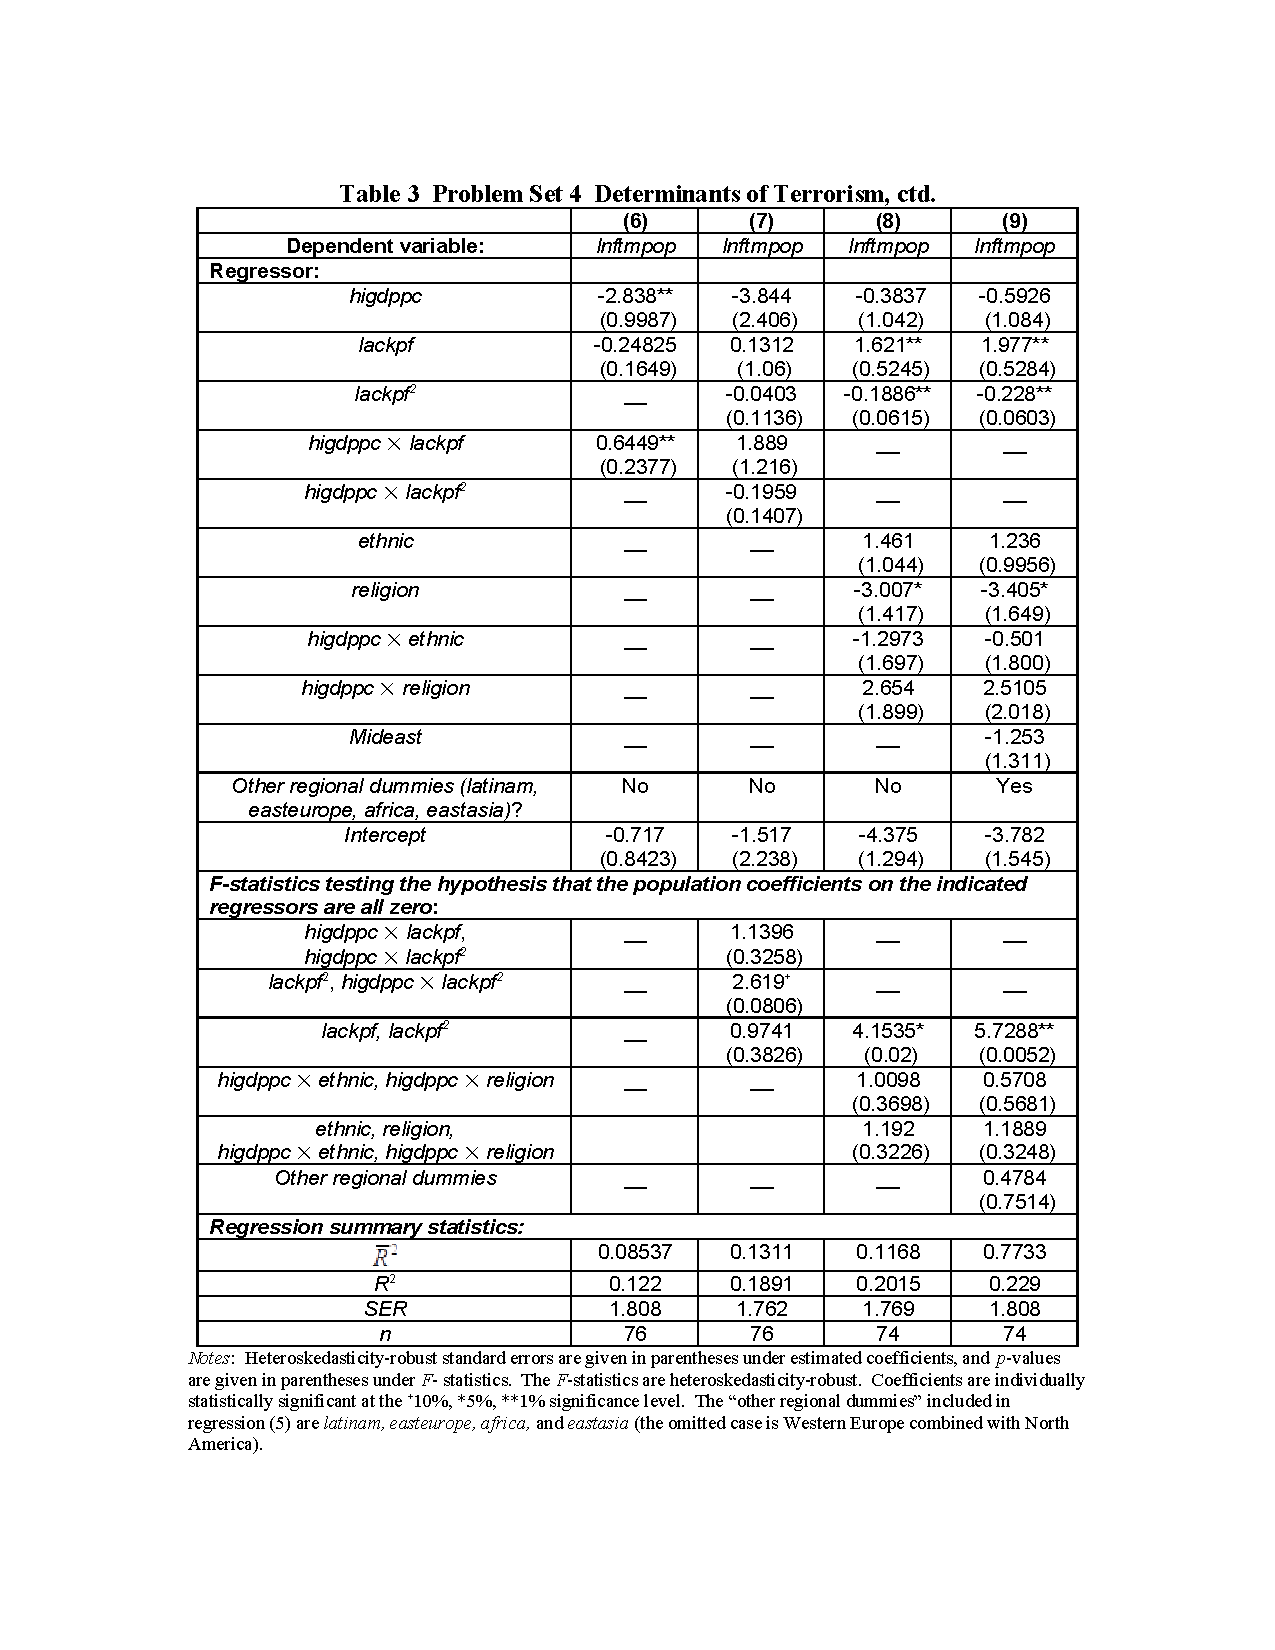
\includegraphics[width=\textwidth]{./figures/table3.pdf}
\end{center}
\break
which has entries given by \verb|R| code
\begin{Verbatim}[fontsize=\small]
t3_reg = list()
t3_reg[[1]] <- robust_lm(lnftmpop ~ higdppc + lackpf +
                           i(higdppc * lackpf), terror_dta)
t3_reg[[2]] <- robust_lm(lnftmpop ~ higdppc + lackpf + i(lackpf ^ 2) +
                           i(higdppc * lackpf) + i(higdppc * lackpf ^ 2), terror_dta)
t3_reg[[3]] <- robust_lm(lnftmpop ~ higdppc + lackpf + i(lackpf ^ 2) +
                           ethnic + religion + i(higdppc * ethnic) + i(higdppc * religion),
                         terror_dta)
t3_reg[[4]] <- robust_lm(lnftmpop ~ higdppc + lackpf + i(lackpf ^ 2) +
                           ethnic + religion + i(higdppc * ethnic) + i(higdppc * religion) +
                           mideast + latinam + easteurope + africa + eastasia, terror_dta)

linearhypothesis(t3_reg[[2]][[1]],
                 c("i(higdppc * lackpf) = 0", "i(higdppc * lackpf^2) = 0"),
                 vcov = vcovhc(t3_reg[[2]][[1]]))
linearhypothesis(t3_reg[[2]][[1]],
                 c("lackpf = 0", "i(higdppc * lackpf^2) = 0"),
                 vcov = vcovhc(t3_reg[[2]][[1]]))
linearhypothesis(t3_reg[[2]][[1]],
                 c("lackpf = 0", "i(lackpf^2) = 0"),
                 vcov = vcovhc(t3_reg[[2]][[1]]))
linearhypothesis(t3_reg[[3]][[1]],
                 c("lackpf = 0", "i(lackpf^2) = 0"),
                 vcov = vcovhc(t3_reg[[3]][[1]]))
linearhypothesis(t3_reg[[3]][[1]],
                 c("i(higdppc * ethnic) = 0", "i(higdppc * religion) = 0"),
                 vcov = vcovhc(t3_reg[[3]][[1]]))
linearhypothesis(t3_reg[[3]][[1]],
                 c("i(higdppc * ethnic) = 0", "i(higdppc * religion) = 0",
                   "ethnic = 0", "religion = 0"),
                 vcov = vcovhc(t3_reg[[3]][[1]]))
linearhypothesis(t3_reg[[4]][[1]],
                 c("lackpf = 0", "i(lackpf^2) = 0"),
                 vcov = vcovhc(t3_reg[[4]][[1]]))
linearhypothesis(t3_reg[[4]][[1]],
                 c("i(higdppc * ethnic) = 0", "i(higdppc * religion) = 0"),
                 vcov = vcovhc(t3_reg[[4]][[1]]))
linearhypothesis(t3_reg[[4]][[1]],
                 c("i(higdppc * ethnic) = 0", "i(higdppc * religion) = 0",
                   "ethnic = 0", "religion = 0"),
                 vcov = vcovhc(t3_reg[[4]][[1]]))
linearhypothesis(t3_reg[[4]][[1]],
                 c("latinam = 0", "easteurope = 0",
                   "eastasia = 0", "africa = 0"),
                 vcov = vcovhc(t3_reg[[4]][[1]]))
\end{Verbatim}

\section*{Problem 6}
\begin{center}
  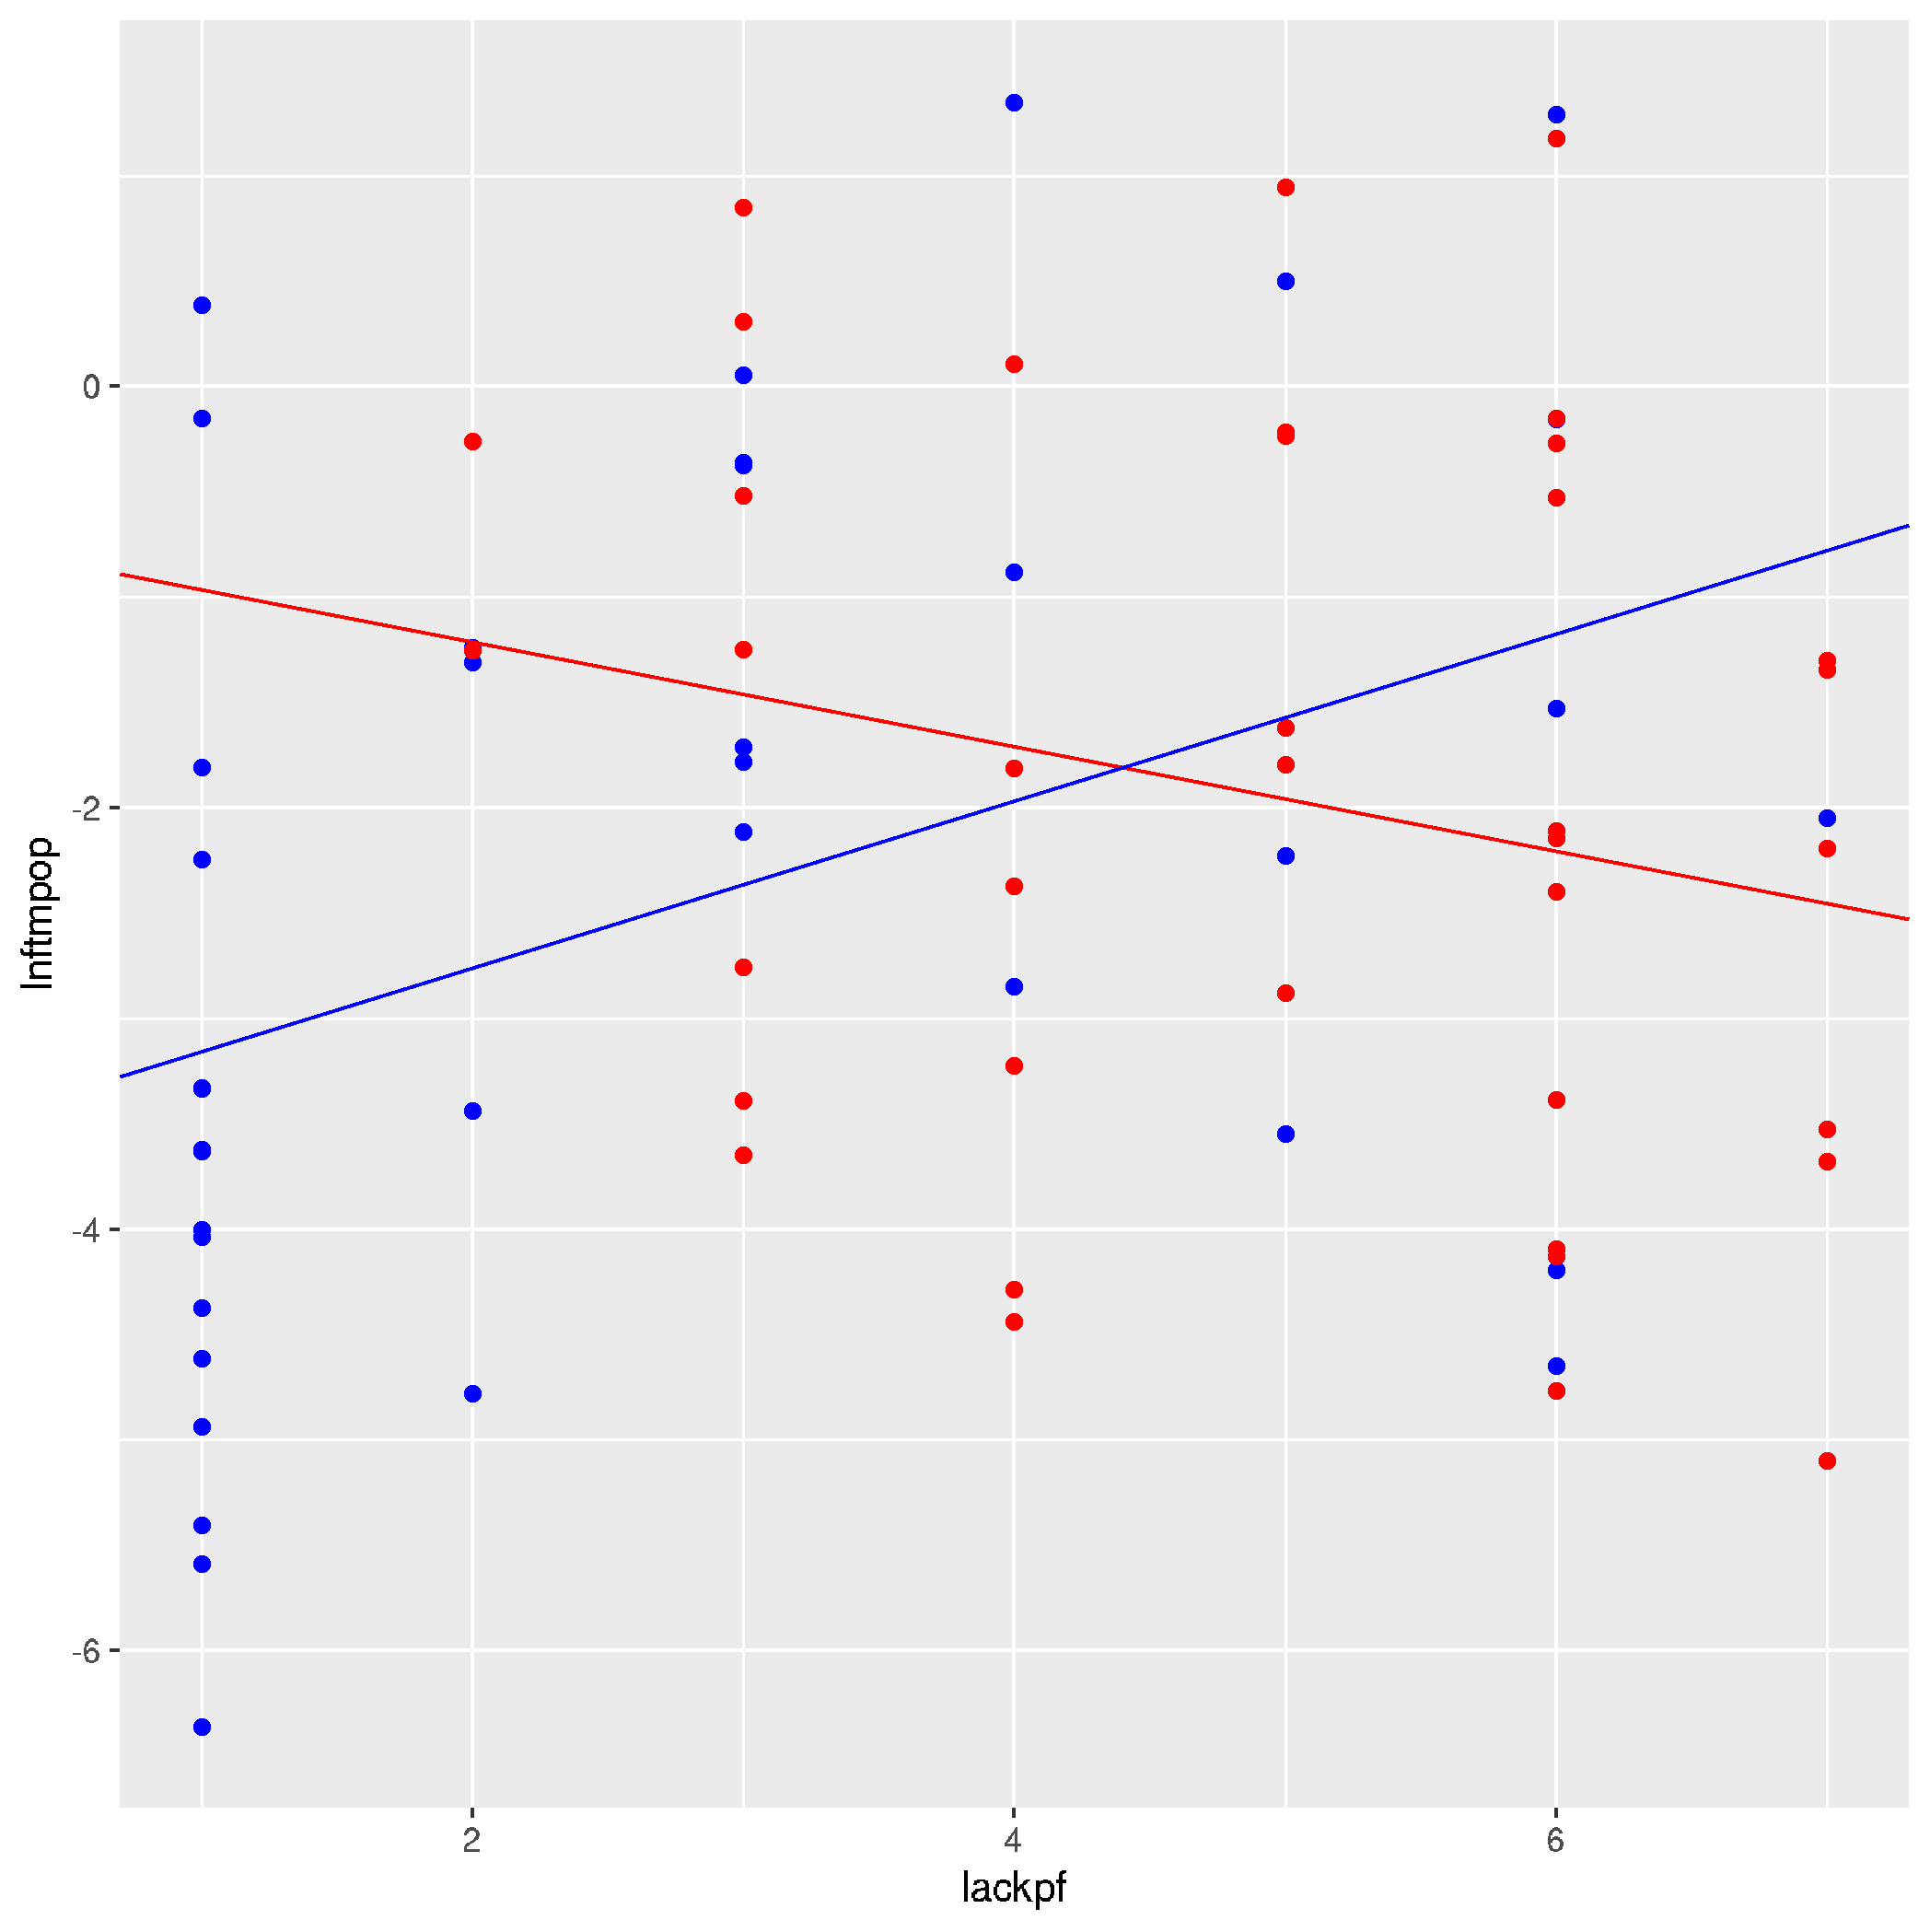
\includegraphics[width=0.6\textwidth]{./figures/6.png}
\end{center}
where blue represents $higdppc = 1$ and red is $higdppc = 0$. This gives linear regression lines of
\begin{align*}
  \begin{cases}
    \log(ftmpop) = -0.717-2.838 + (-0.24825 + 0.6449)lackpf & higdppc = 1\\
    \log(ftmpop) = -0.717 + -0.24825 lackpf & higdppc = 0
  \end{cases}
\end{align*}
where the top comes out to $\log(ftmpop) = -3.555 + 0.39665lackpf$.

This plot is given by
\begin{Verbatim}[fontsize=\footnotesize]
> ggplot(data=terror_dta) +
    geom_point(data=terror_dta[terror_dta$higdppc == 1,], aes(x=lackpf, y=lnftmpop), col="blue") +
    geom_point(data=terror_dta[terror_dta$higdppc == 0,], aes(x=lackpf, y=lnftmpop), col="red")  +
    geom_abline(slope = -0.24825 + 0.6449, intercept=-0.717-2.838, col="blue") +
    geom_abline(slope = -0.24825, intercept=-0.717, col="red")
\end{Verbatim}

\section*{Problem 7}
\subsection*{a}

The difference between the slopes is exactly the coefficient of $higdppc \times lackpf$, which we see is significantly different from zero at a $5\%$ level from the table.

\subsection*{b}

Given the two regression lines, we can interpret regression 6 as showing that in richer countries ($higdppc = 1$) that less freedom correlates with more terrorism since the sign of $\beta_{lackpf} + \beta_{lackpf \times higdppc}$ is positive, but in poorer countries less freedom correlates with less terrorism since the sign of $\beta_{lackpf}$ is negative.

\subsection*{c}

We are testing the statement that the interaction between $higdppc$ and $lackpf$ and between $higdppc$ and $lackpf^{2}$ are both statistically insignificant ($H_{0}:\beta_{higdppc \times lackpf} = \beta_{higdppc \times lackpf^{2}} = 0$) (morally, we test that political freedom has the same effect on terrorism in both rich and poor countries, and if we can reject the null, the rich and poor countries differ in how they are affected by political freedom). This has $F = 1.1396, p = 0.3258 > 0.05$, so we cannot reject the null that there is a difference in poor and rich countries in terms of the effect of political freedom on terrorism.

\subsection*{d}

We are testing the statement that both the interaction between $higdppc$ and $lackpf^{2}$ and $lackpf^{2}$ itself are both statistically insignificant ($H_{0}:\beta_{higdppc \times lackpf} = \beta_{lackpf^{2}} = 0$) (morally, we test whether political freedom has a quadratic effect on terrorism, or if political freedom has different nonlinear effect on terrorism in rich and poor countries). This has $F = 1.1396, p = 0.3258 > 0.05$, so we cannot reject the null that there is both no quadratic effect of freedom and that the quadratic effect is the same between rich and poor countries.

\subsection*{e}

No, they are not, as we have that the joint hypothesis that they all vanish has $F=  0.4784, p =0.7514$ (see table), so we cannot reject the null that they are jointly zero, and they are thus not jointly significant.


\section*{Problem 8}

If it is indeed the case that ethnic and religious diversity are both tolerated more when economic outlooks are good, then we would expect that rich and poor countries have different associations between $lnftmpop$ and $ethnic$ and $religion$. This translates to, in regressions 8 and 9, that we would expect $\beta_{higdppc \times ethnic}, \beta_{higdppc \times religion}$ to be significantly different from 0 (as otherwise economic conditions will not affect ethnic and religious tolerance). However, this isn't the case; the $F-$test that these interaction terms are zero come out as statistically insignificant in both regressions (8: $F = 1.0098, p = 0.369$, 9: $F = 0.5708, p = 0.568$). Further, its not even clear that ethnicity or religious diversity even affect terrorism rates in either case, with the $F-$test that $ethnic, religion$ and their interaction terms still coming out to be jointly insignificant in both regressions.

\section*{Problem 9}

Running the regressions shows that it is hard to predict terrorism from as little information as this; the models that we can draw are enough to prove some priors incorrect, but is unable to give us real siginficant predictive power. For example, the model can show that our expectation that poverty escalates religous and ethnic conflicts into terrorism is not supported by the data, but it can't tell us what things in a country \textit{do} escalate into terrorism. We can only paint broad and unsatisfying strokes, noting, for example, that moderately free societies produce more terrorism deaths than very free and very restrictive nations (perhaps as a result of very free societies not engendering a lot of terrorism, and very restrictive societies not giving people the chance to become terrorists).

\section*{Problem 10}

\subsection*{a}

Yes, this is important, consider for example the average devoutness of religous followers in the country. This is likely correlated with both religous and ethnic diversity (higher devoutness associates with a more monogamous culture in terms of religion and ethnicity in many cases) and very likely determines terrorism rates as well - no one commits terrorism for a diety they're so-so about. Alternatively, political polarization in the country, which might be higher in poorer countries less entrenched in the neoliberal western orbit, could determine terrorism as well.

\subsection*{b}

This is less of a threat, but still possible; for example, religious factionalization might have nonlinear effects, where a state with high diversity sees less terrorism due to more exposure and thus more tolerance, and a state with one religion sees less terroism due to less religous conflict, but states like those in South Asia with two dominant and conflicting religions see the most violence.

\subsection*{c}

Yes, a giant threat: religous diversity and ethnic diversity are not simple things that can be stuffed into a continuous ordered interval between 0 and 1. Similarly, collecting data about terrorist deaths is probably murky: can we trust all states to accurately collect and report data? What even is categorized as terrorism, anyway? (Probably something discriminatory against nonwhite and people and people from the global south!)

\subsection*{d}

Yes, a large threat: we discarded all countries that had no data for $ftmpop$ in the regression. No prior reason to be sure that this is effectively a random sample of countries.

\subsection*{e}

Yes, a threat as well; consider for example something like ethnic diversity drives terrorism $\rightarrow$ terrorism endangers a ethnic minority $\rightarrow$ mass emmigration of said minority $\rightarrow$ lower ethnic diversity.

\end{document}
% LocalWords:  NetID fancyplain LocalWords colorlinks linkcolor linkbordercolor
